\section{文献计量}

文献计量节点吃的是题录表，不是全文。上游可以是上传的导出文件，也可以是爬回来的表；列名不一样也没关系，
节点里有一张列映射，把任意表的列接到它认识的字段上。

\begin{table}[H]\centering
\caption{能识别的文献导出件}
\label{tab:biblio-formats}
\small
\begin{tabularx}{\textwidth}{p{3.0cm}X}
\toprule
来源 & 说明 \\
\midrule
中国知网 & 三种导出按钮都认：RefWorks 文本、NoteExpress、EndNote \\
CSSCI & 文本导出，中文表头 \\
Web of Science & 纯文本全记录、Excel、RIS、BibTeX \\
Scopus & CSV，中英文表头都认 \\
Dimensions & CSV，要选全记录导出 \\
Lens & 学术文献集合的 CSV \\
PubMed & Medline 文本与 CSV 摘要，没有 XML 读法 \\
其他 & RIS、BibTeX、EndNote、NoteExpress \\
\bottomrule
\end{tabularx}
\end{table}

统一之后的列有记录编号、题名、作者、单位、来源期刊、年份、卷期页码、关键词、摘要、参考文献、DOI 与格式，
再按实际数据追加国家、学科、引用次数、使用次数、基金、文献类型、语言。

几条边界是硬性的。知网的 RefWorks 通常没有参考文献，所以引文网络与共被引建不起来；Lens 的专利集合会被拒绝，
它的引用列写的是记录编号而不是引文文本；Web of Science 的 Excel 缺参考文献整列，能建关键词与学科网络，建不了引文网络。

\section{建网与指标}

节点里先选实体。关键词、作者、机构、国家、学科、主题词、基金做共现，文献、作者、期刊做共被引，还有文献耦合与期刊耦合。
共现类只要实体列与年份列，引文类要参考文献列。

\subsection{时间切片}

按年份切片，每片按 TopN、Top 百分比、g-index 或阈值三元组挑选，再合并。可以设回溯年数、最低被引数、引文扩展的阶数。
切片让早年的小网络与近年的大网络都不至于被对方淹没。

\subsection{剪枝}

边太多时图会糊成一团。三种剪法：不剪、最小生成树、Pathfinder。Pathfinder 有三个参数：距离的范数、间接路径最多几跳、保留比例。
默认在每片内部剪完再合并，也可以合并以后一次剪。

\subsection{指标}

每个节点算度、中介中心性、特征向量中心性、PageRank 与 Sigma。输入带被引次数时追加总被引与 h 指数，带使用次数时追加使用次数合计。
中介中心性在节点很多时按抽样估算，控制台会写明抽了多少个源点。

\begin{figure}[H]\centering
\begin{tikzpicture}[scale=0.9]
  \foreach \a/\b in {0/1,0/2,1/2,1/3,2/3,3/4,2/4,4/5,3/5,0/5} {
    \pgfmathsetmacro{\xa}{cos(\a*72+18)*1.9}
    \pgfmathsetmacro{\ya}{sin(\a*72+18)*1.9}
    \pgfmathsetmacro{\xb}{cos(\b*72+18)*1.9}
    \pgfmathsetmacro{\yb}{sin(\b*72+18)*1.9}
    \draw[draw=cA!45,line width=0.8pt] (\xa,\ya) -- (\xb,\yb);
  }
  \foreach \a/\r in {0/0.26,1/0.34,2/0.22,3/0.30,4/0.20,5/0.24} {
    \pgfmathsetmacro{\xa}{cos(\a*72+18)*1.9}
    \pgfmathsetmacro{\ya}{sin(\a*72+18)*1.9}
    \fill[cA!60] (\xa,\ya) circle (\r);
    \draw[draw=cA] (\xa,\ya) circle (\r);
  }
  \node[tag] at (0,-2.4) {圆的大小是频次，线的粗细是共现强度，位置由布局算定};
\end{tikzpicture}
\caption{知识图谱的样子}
\label{fig:kg}
\end{figure}

\subsection{聚类、突现与变异}

聚类用谱聚类，簇数留空时按特征值间隙自动选。簇名可以用 LLR、LSI、互信息或 TF-IDF 生成，也可以用手工标签覆盖。
突现按逐年文档数算，每个节点保留最强的一段区间，另写一张突现词表。结构变异比较相邻两期连边分布的散度，
只有两期都存在的节点才计分，切片不连续时不跨缺口比较。

情感叠加与话题叠加需要上游已经写好的标签列。每个节点追加两列，一列是主导标签，一列是各标签的篇数分布；
分母只算有标签的文档，空白是没有判断，不当中性。

\subsection{输出与图}

默认输出一行一节点的实体表，也能单独输出边表、簇表、突现表与双图叠加表。成图有十四种：知识图谱、环形图、聚类时间线、景观图、
突现词图、时区图、聚类年份热力图、三维图谱、结构变异图、双图叠加、情感叠加、话题叠加、国家地理图、同心环。

每张图都另出一份 TikZ 源与一份三线表。图谱与环形图还带按年份回放：拖动底下那条滑杆，节点按到那一年为止的累计频次长大，
最后一帧与完整图完全一致。

\section{AIGC 的文献计量}

这一段从知网采集开始，到四张图结束。打开“\texttt{AIGC文献计量（知网自动采集3000篇·去重清洗）}”。

\begin{figure}[H]\centering
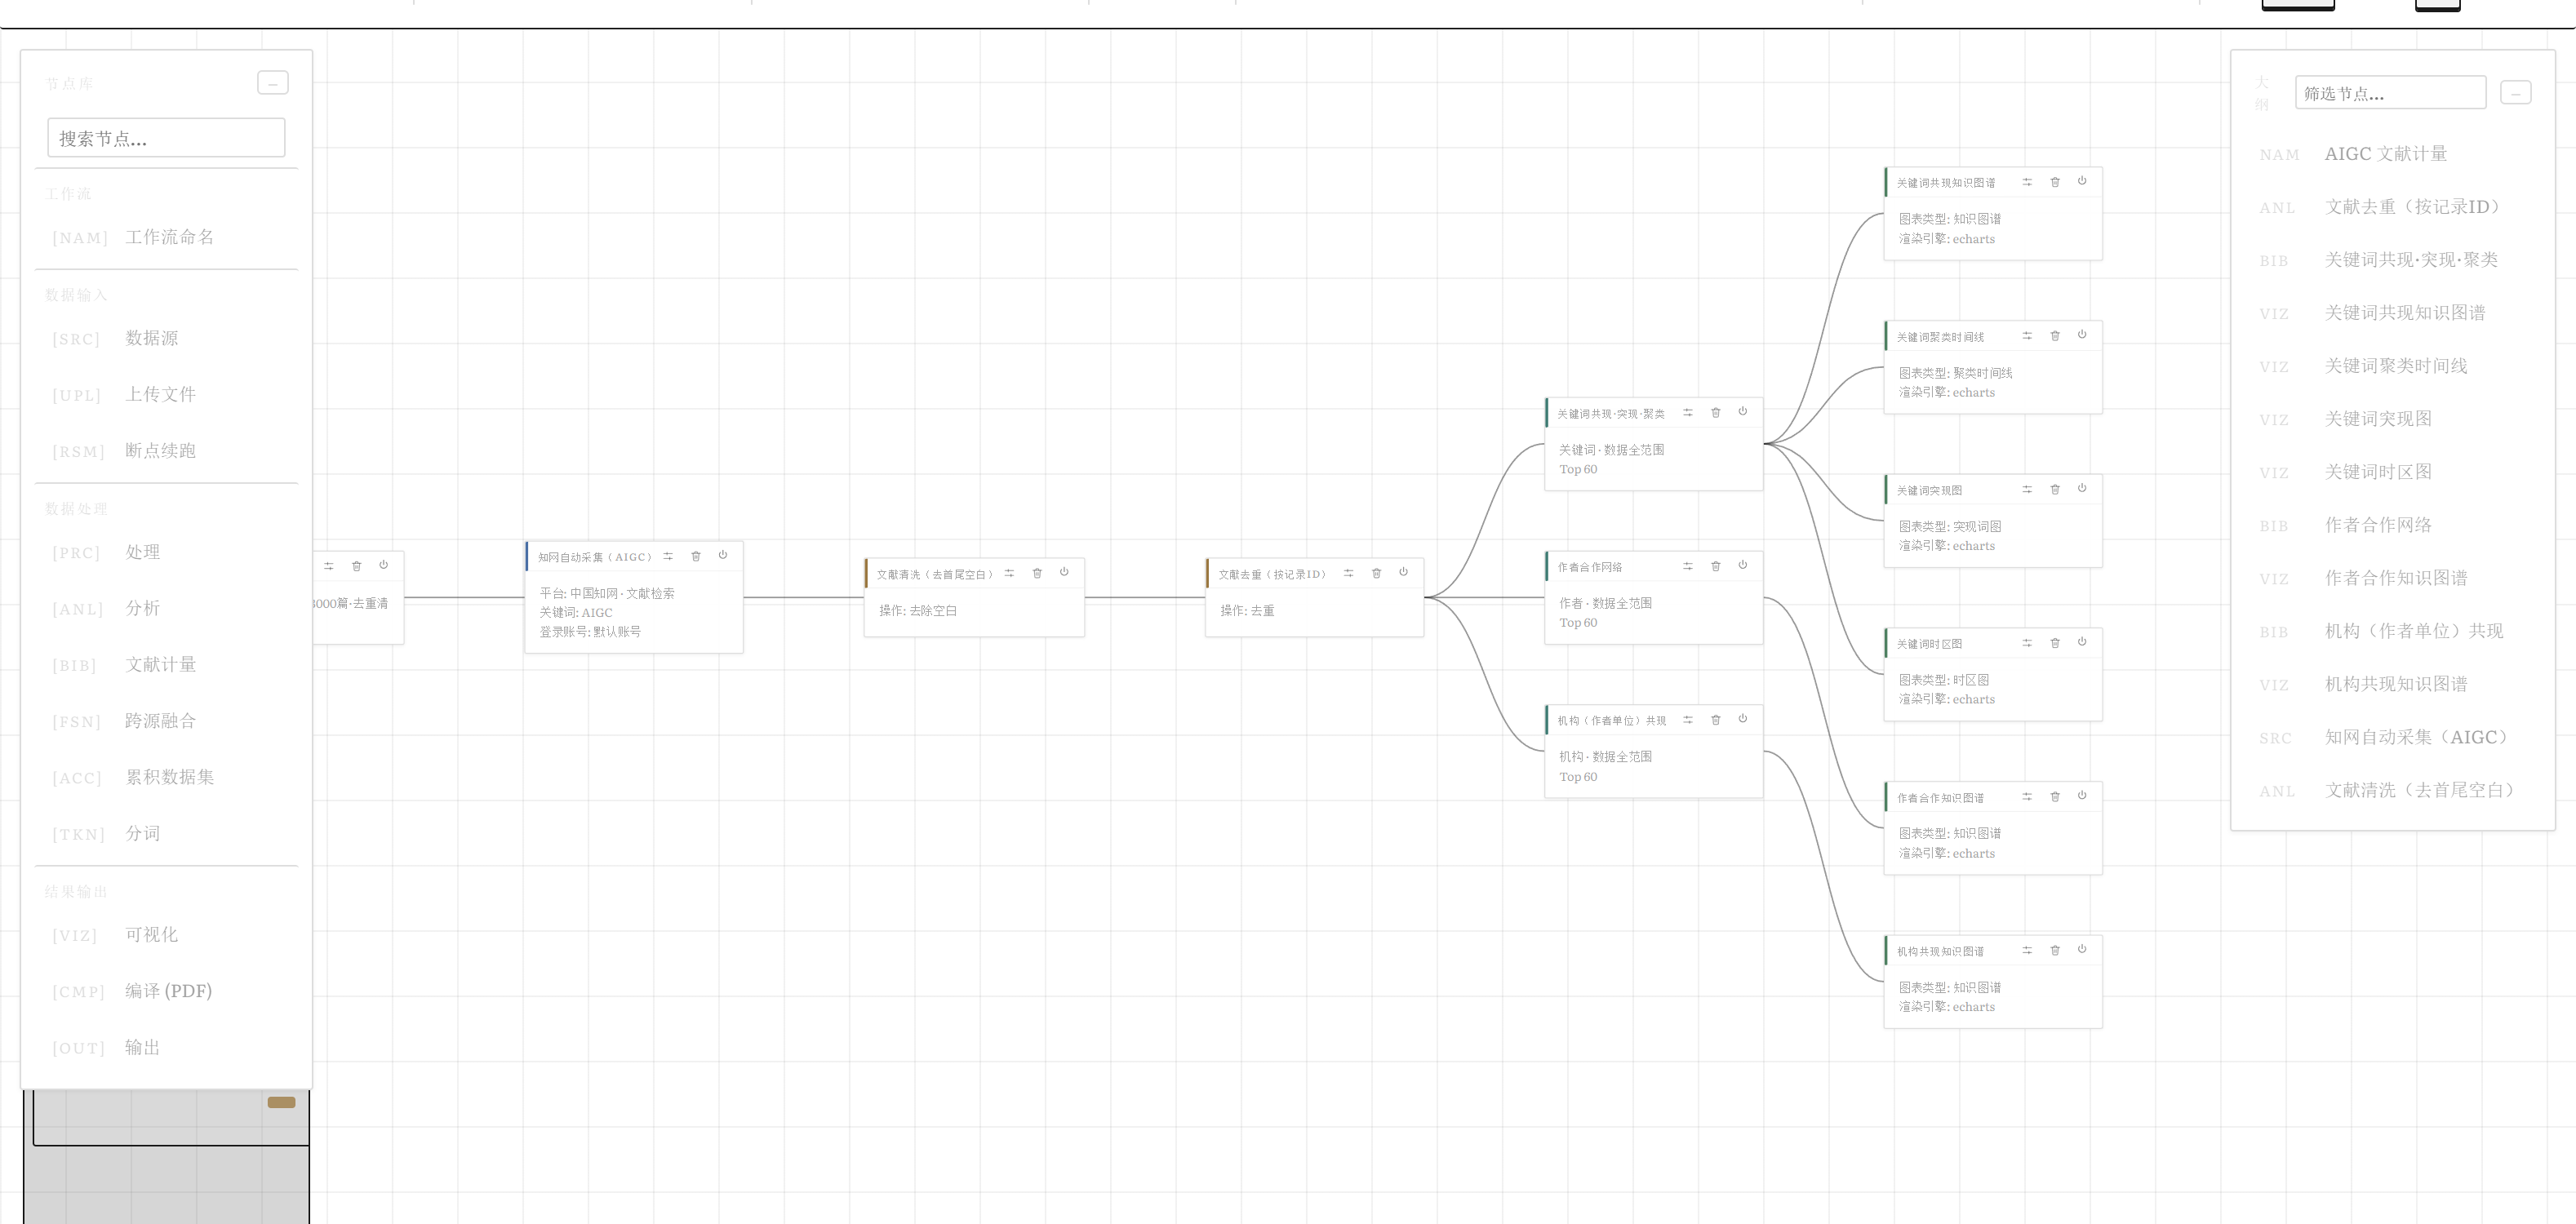
\includegraphics[width=0.98\textwidth]{bib-canvas.png}
\caption{AIGC 文献计量：采集、去重、三路建网、四张图}
\label{fig:bib-canvas}
\end{figure}

\subsection{采集}

数据源选“\texttt{中国知网}”，关键词 \texttt{AIGC}，目标三千篇。知网的全选只作用于当页，程序逐页点一次全选再导出，
所以篇数能走到你填的数。

\subsection{清洗}

采回来的题录先过一遍去重，按记录编号判重；再过一遍去空白，把题名、作者、单位、期刊、关键词、摘要、DOI 这几列的空白去掉。
列名在这里要逐字对上，写错会被拒绝并列出实际有哪些列。

\subsection{建网}

中间那个文献计量节点建关键词网：实体选关键词，最少出现两次，按 TopN 选点，余弦相似度，最小生成树剪枝，按五年切片，开聚类与突现。
输出实体表，同时把图谱、边表、簇表、突现表都写成文件。

\begin{figure}[H]\centering

\includegraphics[width=0.31\textwidth]{bib-node.png}
\caption{文献计量节点：实体、切片、选择、剪枝、聚类都在这一屏}
\label{fig:bib-node}
\end{figure}

右边两个节点分别建作者网与机构网，参数更简单：最少一次，不剪枝，取前六十。三条网共用同一份题录，
所以只要采集与清洗跑过一次，后面可以反复调参数重跑，不用再上站点。

\subsection{出图}

四个可视化节点分别接三条网，图表类型选知识图谱、聚类时间线、突现词图、时区图。每个节点里“\texttt{生成 LaTeX 图}”默认开着，
所以除了屏幕上的图，还会在导出目录留下可以编译的图源。后面可以再接一个编译节点，把图与表合成一份 PDF。

\begin{figure}[H]\centering
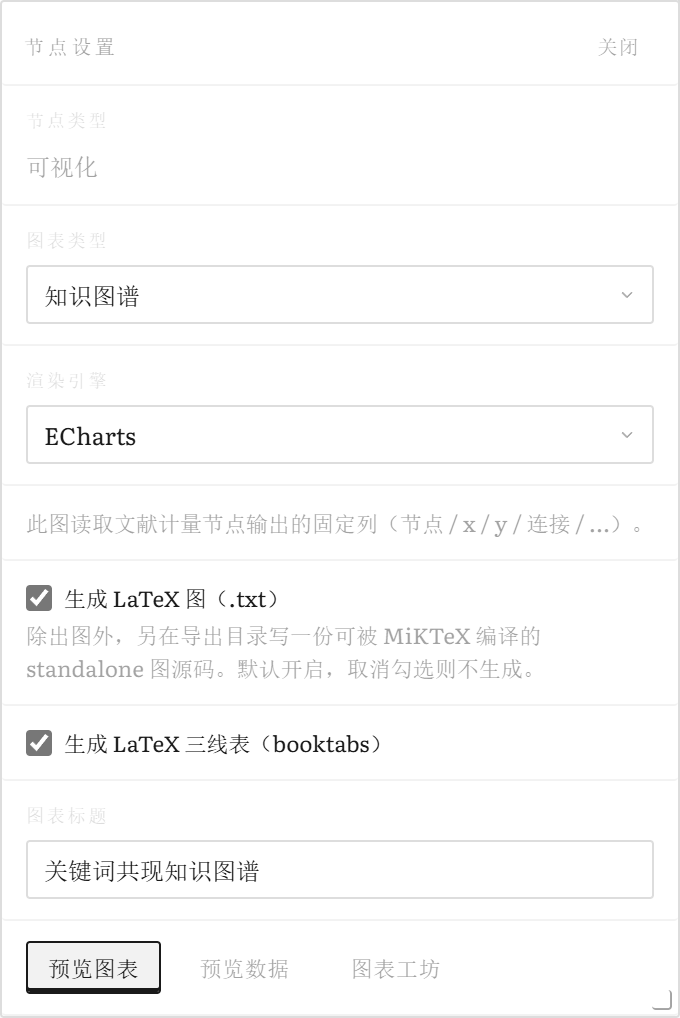
\includegraphics[width=0.31\textwidth]{bib-graph.png}
\caption{可视化节点里的图表类型与 LaTeX 选项}
\label{fig:bib-graph}
\end{figure}

\subsection{跨运行监测}

在文献计量节点里填一个监测项目名，每次运行都会把这张网存成该项目的一份快照，并与上一次对比：
新增与消失的节点、新增与消失的连边、变了的属性、新簇与结束的突现、动过的参数，逐条打印并另存一份表。
配上定时任务，就是一条领域监测线。
